\subsection{Setting and three implementations of one function}
\label{sec:three}

Consider one round of scaled dot-product attention over $N$ agents, per batch
element, with head width $d$. Agent $i$ forms a query $q_i$, and every agent
contributes a key and a value; self-attention is masked. Write
$s_i = q_i K^\top \in \mathbb{R}^N$ for the score vector and
$a_i = \mathrm{softmax}(s_i)$ for the attention weights. Dense attention
computes $m_i = a_i V$.

A top-$k$ variant keeps only the $k$ largest entries of $a_i$ and renormalises.
Crucially, the \emph{same function} admits implementations with very different
costs, and the literature does not consistently distinguish them.

\begin{description}
  \item[\Mask.] Compute $a_i$ in full, multiply by a $\{0,1\}$ mask,
    renormalise, and evaluate $m_i = \tilde{a}_i V$ with $\tilde{a}_i$ still
    dense in memory. The discarded entries are materialised as zeros. Executed
    multiply--accumulates are \emph{identical} to dense, plus the cost of
    selection and masking.
  \item[\Gath.] Take the top-$k$ of the raw scores, softmax over those $k$
    values only, gather the corresponding value rows into a $(B,N,k,d)$ tensor,
    and contract $(B\!\cdot\!N,1,k)\times(B\!\cdot\!N,k,d)$. No zeros are
    materialised and the aggregation genuinely shrinks.
  \item[Fused dense.] Compute the same function as dense through a fused kernel
    \citep{dao2022flashattention,rabe2021selfattention} that never
    materialises the $(B,N,N)$ weight matrix at all.
\end{description}

\begin{figure}[t]
\centering
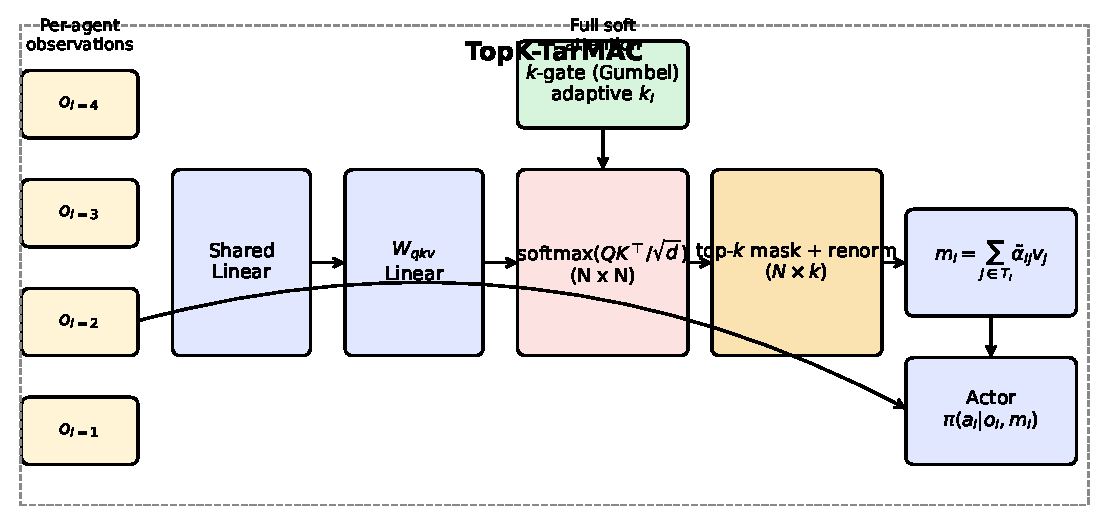
\includegraphics[width=\linewidth]{figures/fig1_schematic.pdf}
\caption{The same top-$k$ attention, computed three ways. All three form the
full score matrix, because selecting peers by score requires every score. They
differ in what happens next: the fused kernel never materialises the weights;
the masked variant stores the discarded entries as zeros and multiplies them
anyway, so its executed operation count equals dense; only the gathered variant
compacts the kept rows and shrinks the product. \textbf{The efficiency claim in
the literature is a claim about the third row.}}
\label{fig:schematic}
\end{figure}

\Gath{} and \Mask{} compute the same function. Two facts make this so:
softmax is monotone within a row, so the top-$k$ weights are the top-$k$
scores; and a softmax over just those $k$ scores equals the dense softmax
restricted to them and renormalised. We verify agreement to $<10^{-10}$ in
\texttt{float64} and pin it with a regression test. \textbf{The efficiency
claim in the literature is a claim about \Gath{}}; benchmarking \Mask{}
measures an implementation artifact, and benchmarking against unfused dense
flatters the sparse method by ignoring what production kernels actually cost.
We therefore report all three throughout.

\subsection{A ceiling on what sparsity can save}
\label{sec:bound}

Counting multiply--accumulates in the two matrix products that constitute
attention, and excluding the shared input and output projections:
\begin{equation}
C_{\text{scores}} = N^2 d, \quad C_{\text{agg}} = N^2 d, \quad
C_{\text{dense}} = 2N^2 d, \qquad
C_{\text{top-}k} = \underbrace{N^2 d}_{\text{all scores}} + \underbrace{Nkd}_{\text{aggregate }k}.
\end{equation}

\begin{proposition}[Ceiling]
\label{prop:ceiling}
For any selection rule that requires the complete score vector of each query,
\begin{equation}
\frac{C_{\text{dense}}}{C_{\text{top-}k}}
= \frac{2N^2 d}{N^2 d + Nkd} = \frac{2N}{N+k} < 2
\qquad \text{for all } k \ge 1,
\end{equation}
with supremum $2$ approached only as $k/N \to 0$. No choice of $k$ or $N$
yields more than a $2\times$ reduction in attention FLOPs.
\end{proposition}

\begin{proof}
$C_{\text{top-}k} > N^2 d = \tfrac12 C_{\text{dense}}$ for every $k \ge 1$
since $Nkd > 0$. The ratio decreases monotonically in $k$ and tends to $2$ as
$k/N \to 0$.
\end{proof}

The commonly reported figure $1 - k/(N-1)$ describes the aggregation term
alone, which is at most half of attention; quoting it as \emph{the} saving
overstates the achievable reduction by a factor approaching two, before any
question of whether it is realised in time.

The assumptions are worth separating, because only one of them is load-bearing.
\textbf{(A1) Single round}: with $R$ rounds both terms scale by $R$ and the
ratio is unchanged. \textbf{(A2) Data-dependent selection}: the kept set is a
function of the scores, so all $N$ scores must be formed. \textbf{(A3) Per
head}: with $H$ heads of width $d/H$ both terms scale identically.
\textbf{(A4) Projections excluded}: including the shared $qkv$ and output
projections moves the ratio strictly closer to $1$, so
Proposition~\ref{prop:ceiling} remains a valid upper bound. \textbf{(A5)
Selection cost excluded}: counting the top-$k$ operation itself can only
decrease the ratio --- and Section~\ref{sec:decomp} shows this term dominates
in practice.

Only A2 lifts the ceiling when it fails.

\begin{proposition}[Escape]
\label{prop:escape}
If the kept set is determined \emph{structurally} --- by information obtainable
without forming the scores, in $o(N^2 d)$ --- then scores need not be computed
for discarded pairs, and
$C_{\mathrm{struct}} = Nkd + Nkd = 2Nkd$, giving
$C_{\text{dense}}/C_{\mathrm{struct}} = N/k$, which is unbounded in $N/k$.
\end{proposition}

Qualifying rules include a fixed communication topology, a spatial or distance
prior, a locality-sensitive hash, and a learned \emph{static} graph. This is
why Longformer and BigBird obtain asymptotic savings where data-dependent
top-$k$ cannot, and it is the concrete design target for any successor method:
\textbf{to beat $2\times$, a method must decide where to look before
looking.} In an environment with spatial structure, a distance-calibrated
selector is the obvious candidate, and we record it as the primary future
direction.

\subsection{Why the ceiling is not the binding constraint}
\label{sec:roofline}

Proposition~\ref{prop:ceiling} bounds a quantity that, in this regime, does not
govern runtime. Attention here is memory-bound, and for memory-bound kernels
time tracks bytes moved, not arithmetic performed
\citep{williams2009roofline}.

We compute arithmetic intensity $\mathrm{AI} = \text{FLOPs} / \text{bytes}$
analytically per stage, counting each tensor read and written once, and compare
it against a \emph{measured} machine balance: a large GEMM gives achievable
FLOP/s, a large device-to-device copy gives achievable bandwidth, and their
ratio is the ridge point above which a kernel is compute-bound. Measuring
rather than quoting datasheet peaks keeps the comparison honest about the
specific device and dtype.

\begin{figure}[t]
\centering
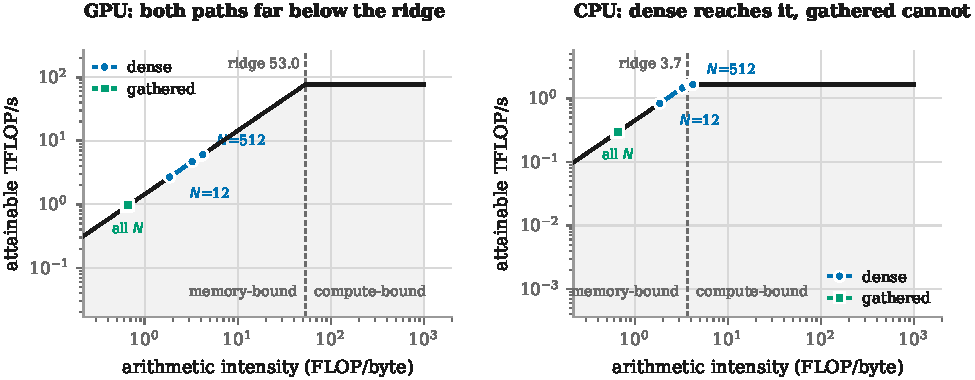
\includegraphics[width=\linewidth]{figures/fig4_roofline.pdf}
\caption{Roofline with \emph{measured} machine balance. On the GPU both paths
sit far below the ridge, so both are memory-bound and removing arithmetic
cannot buy time. On the CPU --- whose balance is an order of magnitude lower
--- the dense path reaches the ridge while the gathered path, pinned at
intensity $0.66$ for every $N$, does not. That asymmetry is why the gap is
\emph{wider} on CPU, not narrower.}
\label{fig:roofline}
\end{figure}

\begin{table}[t]
\centering
\small
\caption{Measured machine balance, and analytic arithmetic intensity of the two
paths at batch $256$, $d{=}16$, $k = 25\%$ of peers. Both paths sit far below
both ridge points, i.e.\ both are memory-bound; the sparse path is
\emph{further} below.}
\label{tab:roofline}
\begin{tabular}{lrrr}
\toprule
\textbf{Device} & \textbf{Achievable GEMM} & \textbf{Achievable bandwidth} & \textbf{Ridge point} \\
\midrule
RTX PRO 6000 Blackwell (\texttt{fp32}) & 76.8 TFLOP/s & 1448.8 GB/s & 53.0 FLOP/byte \\
x86\_64 CPU (\texttt{fp32})            & 1.66 TFLOP/s & 450.8 GB/s  & 3.68 FLOP/byte \\
\midrule
\textbf{$N$} & \textbf{dense AI} & \textbf{gathered AI} & \textbf{ratio} \\
\midrule
12  & 1.85 & 0.64 & 0.34$\times$ \\
48  & 3.23 & 0.66 & 0.20$\times$ \\
192 & 3.98 & 0.66 & 0.17$\times$ \\
512 & 4.18 & 0.66 & 0.16$\times$ \\
\bottomrule
\end{tabular}
\end{table}

Table~\ref{tab:roofline} and Figure~\ref{fig:roofline} give the result. The gathered path adds two stages
that move substantial memory for \emph{zero} arithmetic --- the top-$k$
selection and the gather --- so its intensity is pinned near $0.66$ and does
not improve with $N$. At $N{=}512$ the sparse path moves $4.16$\,GB to perform
$2.76$\,GFLOP, against dense's $1.11$\,GB for $4.63$\,GFLOP: $3.8\times$ the
traffic for $0.6\times$ the arithmetic. Removing multiply--accumulates from a
memory-bound kernel does not make it faster, and adding traffic to one makes it
slower.

This also predicts that the result should be architecture-independent, since it
follows from the ratio of the two paths' intensities rather than from any
device constant. Section~\ref{sec:measurement} confirms it on a CPU whose
machine balance differs from the GPU's by more than an order of magnitude.
